In this section we will discuss the basics of the Bitcoin transaction protocol.
We will find definitions which we will use later in section~\ref{sec:atom:atomic-swap} to construct an atomic swap protocol.
The main reference of this section is the book Mastering Bitcoin by Andreas Antonopoulos~\cite{antonopoulos2014mastering}.

\subsection{Bitcoin Transaction Protocol}\label{subsec:pre:bitcointx}

A \emph{Bitcoin Transaction} is a data structure which allows transferring value between participants of the network.
In Bitcoin there are no user balances or user accounts, instead the UTXO model (unspent transaction outputs) is empoloyed.
An UTXO is a output constructed in a previous transaction which holds value in the form of an amount expressed in
Bitcoin (more precisely in Satoshis, which is the smallest unit of Bitcoin) and a locking condition (referred to as
scriptPubKey).
Unspent means that this output has not been spent yet in a transaction and its funds are therefore available to be redeemed by a participant capable of unlocking the output.
To unlock this value one has to provide a script fulfilling the locking condition, referred to as scriptSig.
In the most common case the lock condition will be to provide a valid signature under a public key.
This is referred to as a P2PK or P2PKH output which we will see in more detail in section~\ref{sec:pre:bitcoin:p2pk}.
However, more complex conditions, such we shall see in section~\ref{sec:pre:bitcoin:p2sh} are possible.

\begin{definition}[Unspent Transaction Output - UTXO] An unspent transaction output is a data structure
consisting of a locking condition $\varScriptPubKey$, a value expressed in Bitcoin $\varValue$ and an unlocking script $\varScriptSig$ which is
initially empty and has to be provided by the owner when spending the UTXO in a transaction. In this paper we
generally use $\varUTXO$ to refer to a singular UTXO and $\varUTXOSet$ to refer to a set of UTXOs.
    \[ \varUTXO \opAssign \{ \varValue \opSeperate \varScriptPubKey \opSeperate \varScriptSig \} \]
\end{definition}

We define three auxiliary functions for the creation, spending and verification of an UTXO.
Note that we use $\procVerfId$ as a generalization of a verification function.
In practice verifcation of a UTXO will most of the time correspond to the verification of a digital signature.
However, as we shall see in~\ref{sec:pre:bitcoin:p2sh} this is not necessarily always the case.

\begin{center}
    \fbox{
    \begin{varwidth}{\textwidth}
        \procedure[linenumbering]{$\procCreateUTXO{\varValue}{\varScriptPubKey}$} {
        \pcreturn \varUTXO \opAssign \{ \varValue \opAssign \varValue, \varScriptPubKey \opAssign \varScriptPubKey,
        \varScriptSig \opAssign \cnstEmptySet \}
        } \\
        \procedure[linenumbering]{$\procSpendUTXO{\varUTXO}{\varScriptSig}$} {
        \{ \varValue, \varScriptPubKey \} \opFunResult \varUTXO \\
        \pcreturn \varUTXO \opAssign \{ \varValue \opAssign \varValue, \varScriptPubKey \opAssign \varScriptPubKey,
        \varScriptSig \opAssign \varScriptSig \}
        } \\
        \procedure[linenumbering]{$\procVerfUTXO{\varUTXO}$} {
        \{ \varValue, \varScriptPubKey, \varScriptSig \} \opFunResult \varUTXO \\
        \pcreturn \procVerf{\varScriptPubKey}{\varScriptSig}{\varValue}
        }
    \end{varwidth}
    }
\end{center}

Now a full transaction consists of one, or many UTXOs as inputs and one or many UTXOs as output.
For the transaction to be considered valid the $\varScriptSig$ fields in the inputs need the be correctly filled, and the value in the newly created output UTXOs must not exceed the value stored in the spending UTXOs.
A value lower than what is provided in the inputs is allowed, this means the miner of the transaction gets to collect the difference as a fee.
The higher this fee, the more incentive the miners will have to include your transaction in the blockchain.
Additionally a transaction consists of a version number, and a locktime field which semantically means that a
transaction will only be seen as valid after a certain block number in the Bitcoin blockchain was mined.
Figure~\ref{fig:btc-tx} shows a decoded Bitcoin transaction.

\begin{definition}[Bitcoin Transaction]
    A Bitcoin transaction consists of a series of input UTXOs $\varBtcInputs$, a series of output UTXOs $\varBtcOutpus$, a
    transaction version $\varVersion$, and an optional locktime $\varTime$:
    \[ \varBtcTx \opAssign \{ \varVersion, \varTime, \varBtcInputs, \varBtcOutpus \} \]
\end{definition}

\begin{figure}
    \begin{center}
        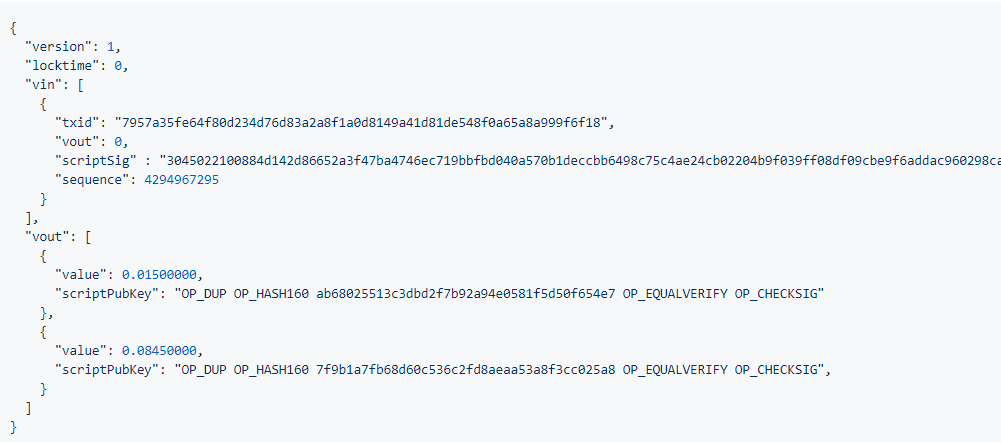
\includegraphics[width=\textwidth]{btc-tx.png}
    \end{center}
    \caption{A decoded Bitcoin transaction~\footcite{https://github.com/bitcoinbook/bitcoinbook/blob/develop/ch06.asciidoc} \label{fig:btc-tx}}
\end{figure}

A transaction is valid if the follwing conditions are fullfilled:

\begin{itemize}
    \item The total value of inputs is greater or equal the total value of outputs.
    \item For all $\varUTXO \opIn \varUTXO$ $\procVerfUTXO{\varUTXO} \opEqNoQ 1$ must hold.
    \item All input UTXOs have not been spent before.
    \item If a locktime $\varTime$ is given, the current block on the Bitcoin blockchain needs to be higher or equal $\varTime$.
\end{itemize}

\begin{definition}[Bitcoin Transaction Scheme]
    We define a Bitcoin Transaction scheme as a tupel of three DPT functions $(\procBuildTransactionId,
    \procSignTransactionId, \procVerfTransactionId)$.
    \begin{itemize}
        \item $\varBtcTx \opFunResult \procBuildTransaction{\varBtcInputs}{\varBtcOutpus}{\varVersion}{\varTime}$: The
        transaction building algorithm is a DPT function which takes as input a set of unspent transaction outputs
        $\varBtcInputs$, a set of newly created transaction outputs $\varBtcOutpus$ a version number $\varVersion$
        and a optional locking time $\varTime$. The algoritm will output an unsigned transaction $\varBtcTx$.
        \item $\funStar{\varBtcTx} \opFunResult \procSignTransaction{\varBtcTx}{\funArray{\varScriptSig}}$: The transaction
        signing algoritm is DPT function which takes as input a unsigned Bitcoin transaction $\varBtcTx$ and an array
        of unlocking scripts $\funArray{\varScriptSig}$ for all inputs of the transaction. The algoritm outputs a
        signed Bitcoin transaction which can now be broadcast to the network.
        \item $\{ 1,0 \} \opFunResult \procVerfTransaction{\varBtcTx}$: The verification algorithm is a DPT function
        taking as input a transaction $\varBtcTx$ outputing 1 on a successfull verification or 0 otherwise. The
        function will check the well-balancedness of the transaction, verify the unlocking scripts, locktime
        as well as scanning through the blockchain if all inputs are indeed unspent.
        Note that any public verifier with access to the blockchain ledger and $\varBtcTx$ will be able to perform the verification.
    \end{itemize}
\end{definition}

Following we will outline two common structures of Bitcoin outputs the P2PK/P2PKH and the P2SH outputs.

\subsubsection{P2PK, P2PKH\label{sec:pre:bitcoin:p2pk}}

P2PK stands for Pay-to-Public-Key and P2PKH for Pay-to-Public-Key-Hash.
In this type of output $\varScriptPubKey$ will be constructed such that its value unlocks if a correct signature is
provided in $\varScriptSig$ for a corresponding public key $\varPubKey$.
P2PKH is an update to this script in which the $\varScriptPubKey$ contains a hashed version of the public key $\varPubKey$,
instead of the public key itself.
To spend a P2PKH output one has to provide the unhashed public key in addition to a valid signature.
This type of output, is the most commonly used output in the Bitcoin blockchain to transfer value from one participant to another.
Delgado et at. found in their paper Analysis of the Bitcoin UTXO set from 2017 that more then 80\% of the UTXO set at
that time consisted of P2PKH transactions, whereas about 17\% were P2SH and 0.12\% P2PK outputs.
~\cite{delgado2018analysis}
P2PKH outputs can be encoded into a Bitcoin address using base58 encoding.
This addresses can be handed out to request a payment from somebody.

\subsubsection{P2SH} \label{sec:pre:bitcoin:p2sh}

If more advanced spending conditions, such as multi signature are required, P2SH (Pay-to-script-hash), introduced in
2012, is a way to implement those in a space efficient and simple matter.
Here the locking condition $\varScriptPubKey$ does not contain a script, but instead the hash of a script.
Upon spending the spender has to provide the original script as well as the unlocking requirements for the script
itself.
Upon verification the hash of the provided script will be computed and compared with the value given in the locking
condition, if those match the actual script will be executed.
The advantages of using this approach over just handcrafting a custom locking script is that the locking scripts are
rather short making the transactions smaller and therefore reducing fees, or rather shifting the fees from the sender
to the owner of the output.
Additionally this type of output can be encoded again into a Bitcoin address similar to a P2PKH output, making it
easy to request a payment.